\defcitealias{StateOfFtd20}{StateOfFtd20}
\defcitealias{StateOfJS21}{StateOfJS21}
\defcitealias{AnReVue22}{AnReVue22}
\section{Editor} \label{sec:editor}

As mentioned before, the \textit{Editor} should be a piece of software facilitating the process of creating and editing a web automation file.

While we designed the workflow definition format to be as readable and concise as possible, the strict JSON syntax makes the format hard to write manually.
Especially less technical users - such as the model user role \hyperref[UserUserRole]{\textit{User}} - could experience difficulties when trying to edit 
larger automation files. 
As stated in the \hyperref[requirements]{Requirements}, the \textit{Editor} should also provide performance-oriented features,
targetting more experienced users - such as the model \hyperref[DevUserRole]{\textit{Developer}}.

\subsection{Technologies}
In accordance with the nonfunctional requirements for the \textit{Editor}, the \textit{Editor} app should be user friendly and easy to use.
Due to its relatively lightweight nature, it is possible to implement the \textit{Editor} as a web application. 

This approach would be beneficial for several reasons - removing the need for installation, providing a cross-platform solution and speeding up the development and debugging process, to name a few.
Implementing the \textit{Editor} as a client-side web application in JavaScript seems like a sensible option also because it might later share a part of the codebase with the \textit{Runner} application.

\subsubsection{Frontend Framework}

Client-side web applications are now seldom developed using plain JavaScript - most developers utilize frontend frameworks and libraries for easier manipulation with the \ac{DOM} tree and state management \citepalias{StateOfFtd20}.

According to a popular 2021 JavaScript developer survey \citepalias{StateOfJS21}, the most popular \ac{JS} frontend frameworks among developers are \textit{React}, \textit{Angular} and \textit{Vue.js}.
While the popularity of the tools changes over time with new emerging technologies coming every year, because of their large following, the aforementioned tools have a large number of third-party libraries 
and modules. Compared to some less popular tools, these frameworks also have better documentation and are better debugged.

When comparing the frameworks against each other, \textit{React} comes off as the framework with the steepest learning curve while being only slightly less popular than \textit{Vue.js}, based on the GitHub stars of the project \citepalias{AnReVue22}.
While all the frameworks are utilizing the model of reusable components, \textit{Angular} and \textit{Vue.js} are taking the concept a little further with their internal \acs{HTML} templating systems.

\textit{React} is the only framework of those three utilizing \acs{JSX}, i.e. combining the \acs{HTML} syntax with the \acs{JS} syntax. 
While this might pose certain difficulties for developers learning this framework, it allows them to interleave the \acs{HTML} and \acs{JS} code in a way that is more readable and easier to maintain in the end.

Since the \textit{Editor}, given the \hyperref[requirements]{requirements}, should not require any advanced features of \textit{Angular} and \textit{Vue}, 
we can utilize the \textit{React} framework for the \textit{Editor}.

\subsection{UI design}

This subsection describes the specific \acs{UI} design and presents mockups for the \textit{Editor} application.
The designs presented here should adhere to the nonfunctional requirements of user-friendliness and ease of use.

These mock-ups are meant to be used as a guide for the \textit{Editor} application implementation.

Please note that the following images do not represent the finished software, only the UI mock-ups.
The mock-up designs are also available in \textit{Figma}\footnote{\href{https://www.figma.com/file/gzisxDDNZX8vbvMdOjfMjT/wbr-editor}{https://www.figma.com/file/gzisxDDNZX8vbvMdOjfMjT/wbr-editor}} for further inspection and future reference.

\clearpage
\begin{figure}[!h]
    \begin{center}
        \fbox{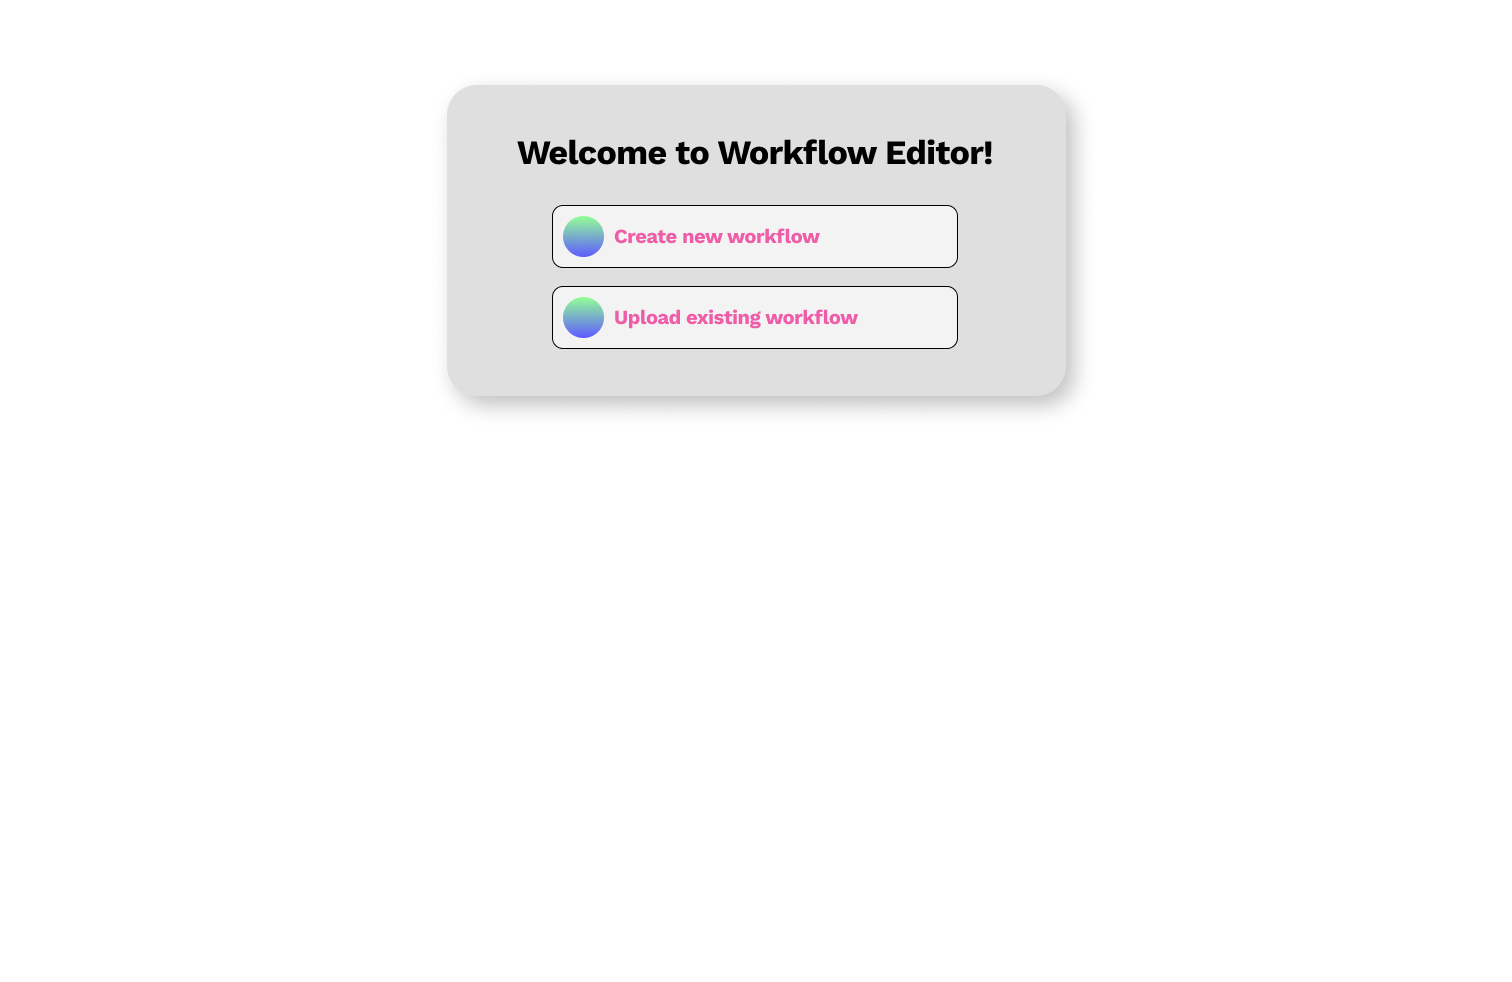
\includegraphics[width=0.8\textwidth]{./img/UIDesigns/Frame 6.png}}
    \end{center}
    \caption{The initial screen}
\end{figure}

As described in the use case analysis, the initial screen of the application should allow the user to create a new blank automation file, or to load an existing automation file.
Choosing to load an existing automation file opens a file selection dialog, allowing the user to select an file from their local file system.

\begin{figure}[!h]
    \begin{center}
        \fbox{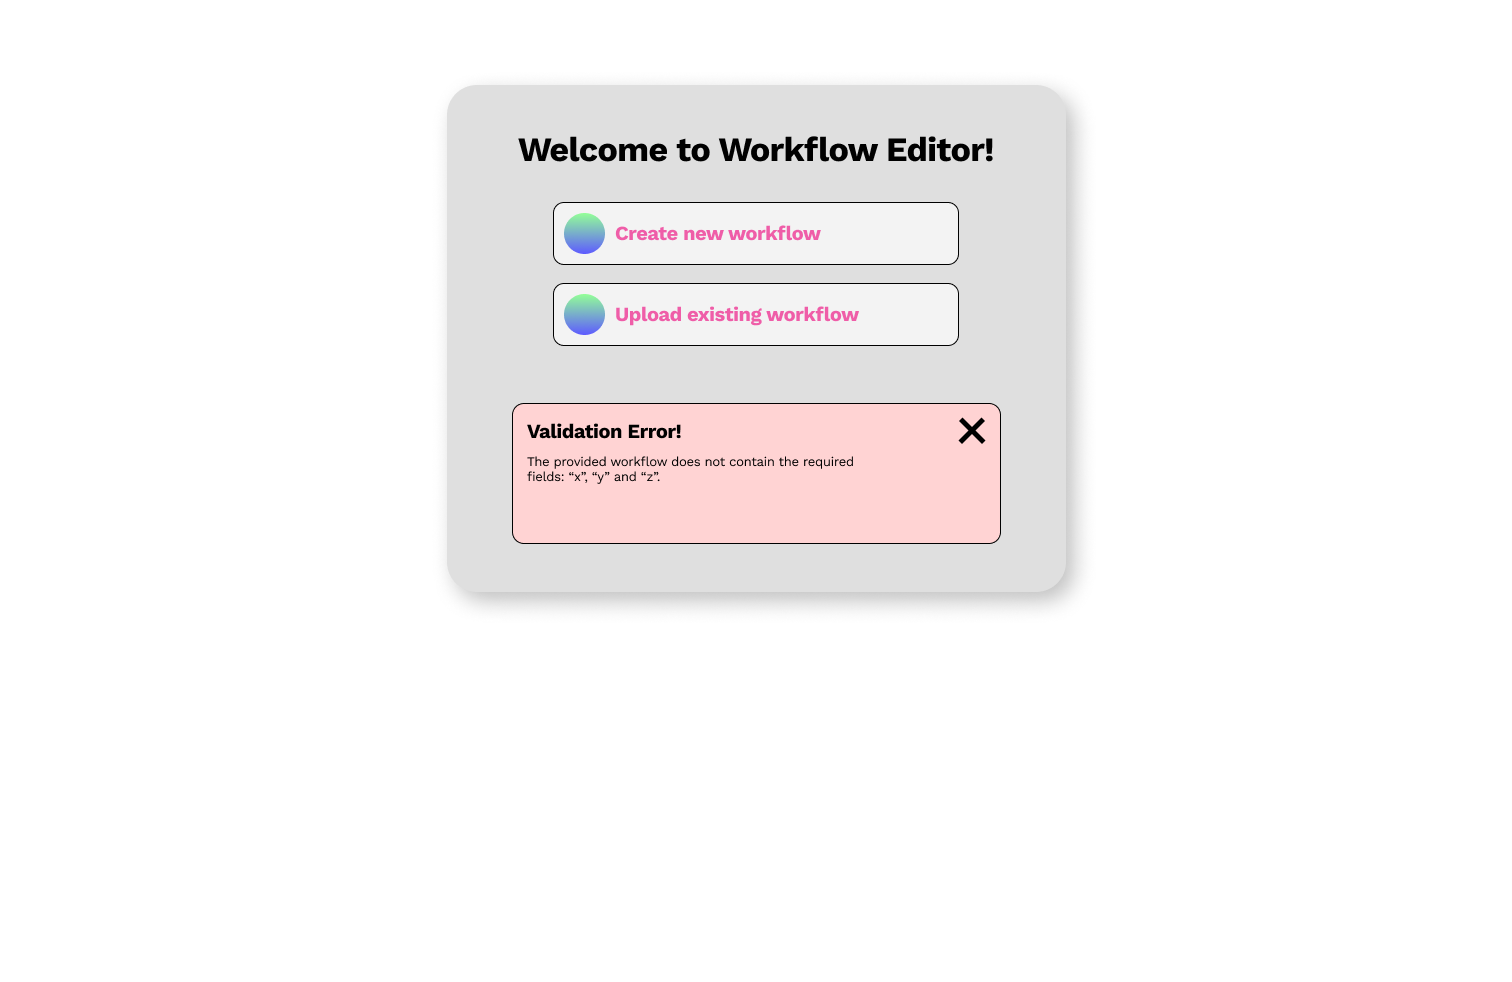
\includegraphics[width=0.8\textwidth]{./img/UIDesigns/MacBook Pro 14_ - 2.png}}
    \end{center}
    \caption{Validation error message}\label{fig:editor-load}
\end{figure}
While creating a new blank file immediately opens the \textit{Editor} application, an uploaded file needs to be validated first - in accordance with the \hyperref[requirements]{functional requirement} 1.2.1.1.2.
If the provided file is not a valid workflow definition file, the user should be notified (\autoref{fig:editor-load}) and the application should remain open, allowing the user to provide different file or to create a new blank file.
\clearpage

\begin{figure}[h!]
    \begin{center}
        \fbox{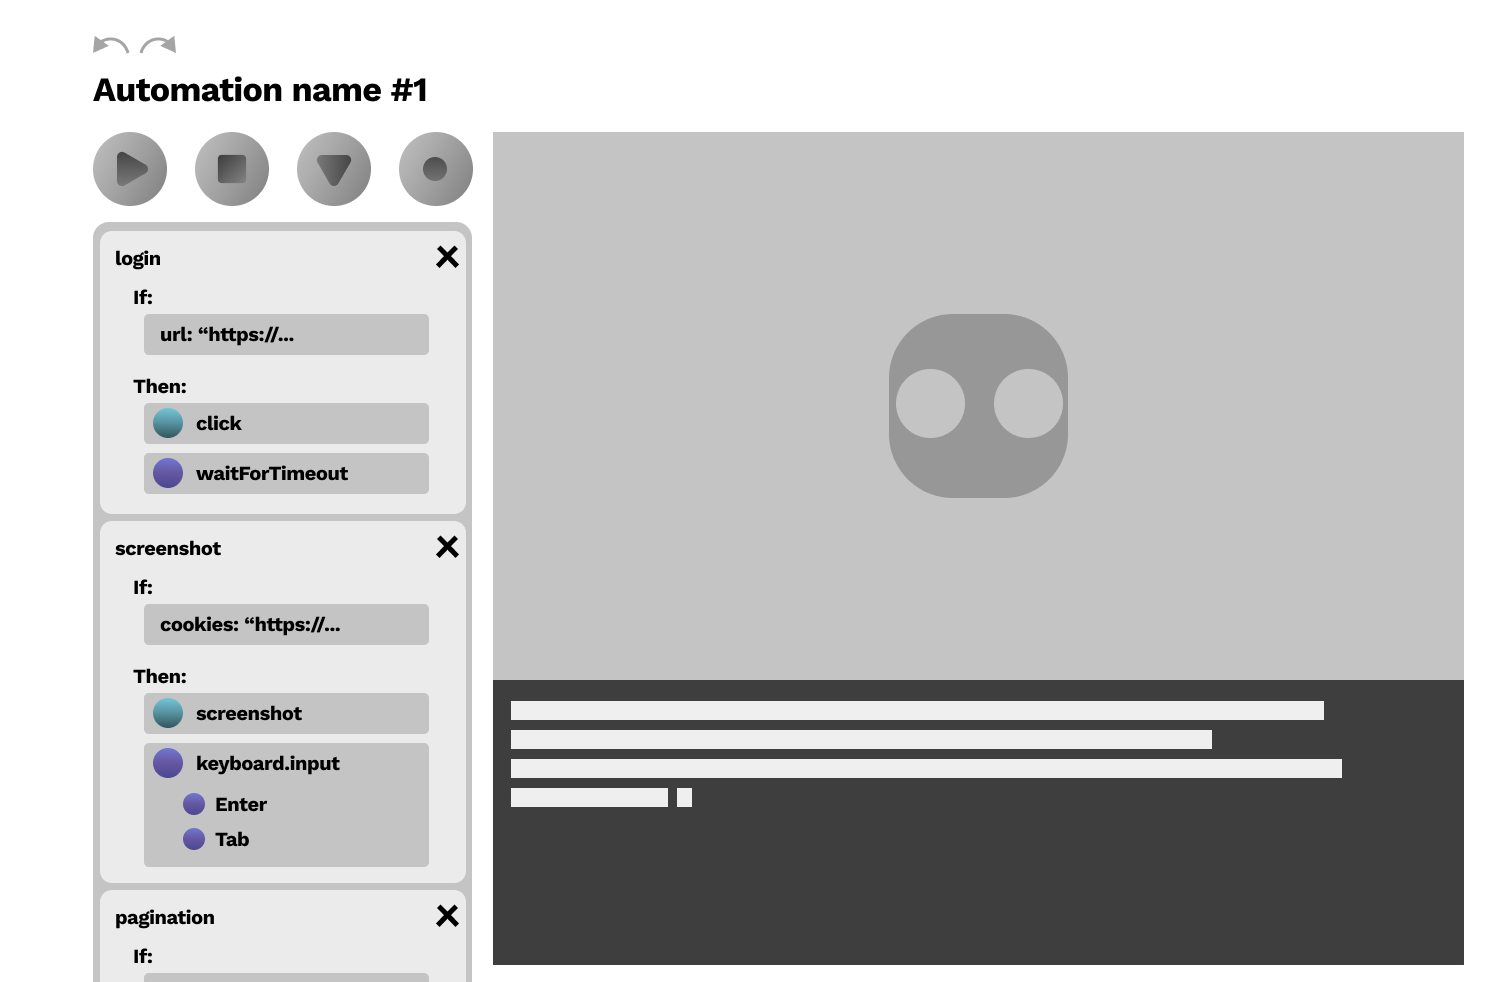
\includegraphics[width=0.8\textwidth]{./img/UIDesigns/MacBook Pro 14_ - 3.png}}
    \end{center}
    \caption{Workflow editor interface} \label{fig:editor-workflow}
\end{figure}

After successfully opening a workflow definition file, the user is presented with the \textit{Workflow editor} interface. 
Here, the user can edit the workflow definition file using a \ac{GUI} editor - in the \autoref{fig:editor-workflow}, the workflow is presented in the left column.

The workflow editor contains a number of \ac{GUI} elements allowing the user to edit the workflow definition file in an intuitive way.
All the actions performed by the user using these tools maintain the proper workflow definition syntax, as required by the \hyperref[requirements]{functional requirement} 1.2.1.1.3.

The hierarchical structure of the workflow definition file allows us to present the workflow in a tree-like, collapsible structure, further enhancing the \ac{UX} of the application.

\begin{figure}[h!]
    \begin{center}
        \fbox{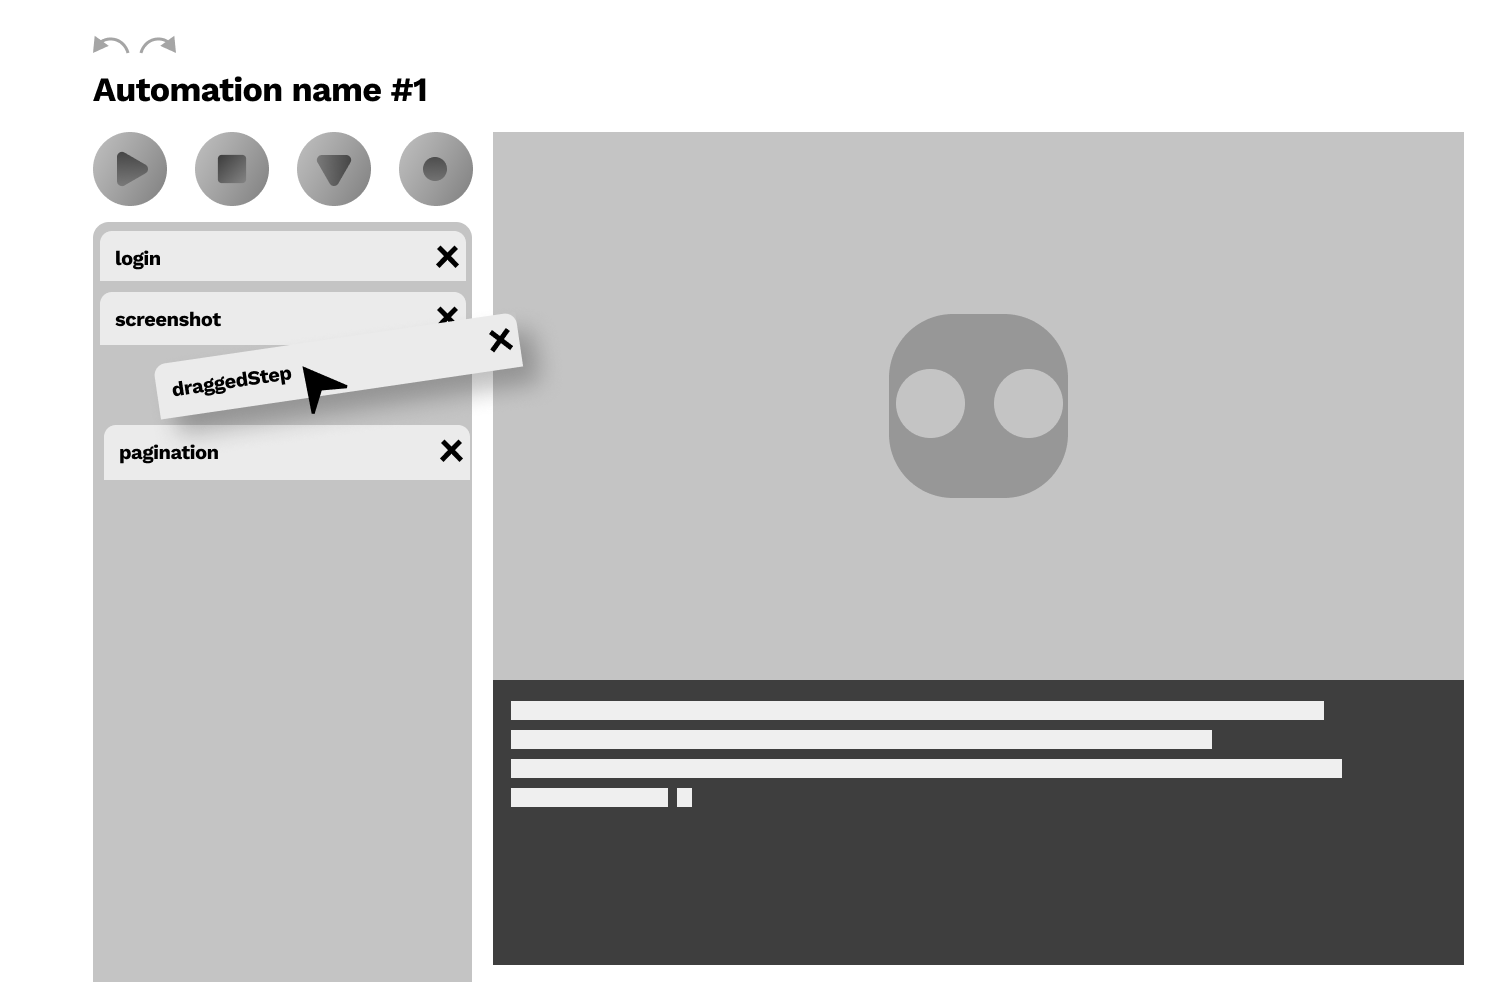
\includegraphics[width=0.8\textwidth]{./img/UIDesigns/MacBook Pro 14_ - 4.png}}
    \end{center}
    \caption{Drag \& Drop controls}
\end{figure}
\clearpage

After finishing the editing of the workflow definition file, the user can test the workflow by clicking the \textit{Run} button.
While this is not required by any of the \hyperref[requirements]{functional requirements}, it is a crucial feature for an editor to have.

In the \autoref{fig:editor-run}, the execution control buttons are located above the workflow editor column. 
The browser window showing the progress of the automation is in the right half of the screen.
Below this window, there is a console for the user to view the output of the automation and debugging information.

During the automation execution, the \textit{Editor} application can highlight the current step of the workflow, allowing the user to follow the execution progress.

\begin{figure}[h!]
    \begin{center}
        \fbox{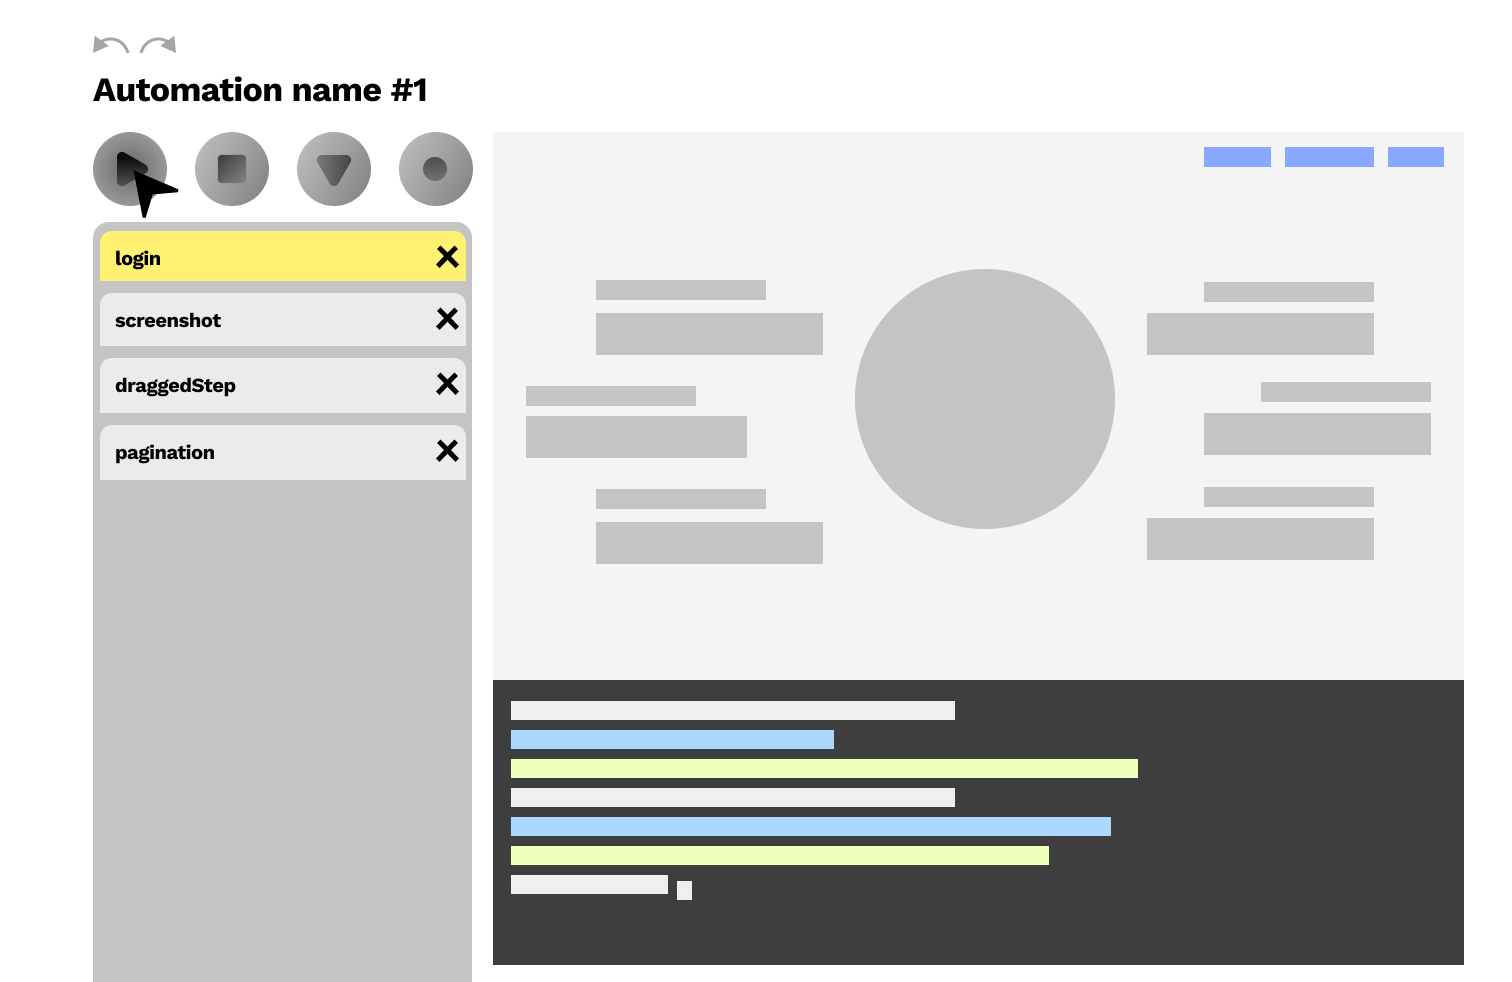
\includegraphics[width=0.8\textwidth]{./img/UIDesigns/MacBook Pro 14_ - 5.png}}
    \end{center}
    \caption{Workflow execution} \label{fig:editor-run}
\end{figure}